% Mecánico rotacional: eje flexible (resorte torsional K entre dos inercias)
\documentclass[border=5pt]{standalone}
\usepackage{tikz}
\usetikzlibrary{arrows.meta, decorations.pathmorphing}
\begin{document}
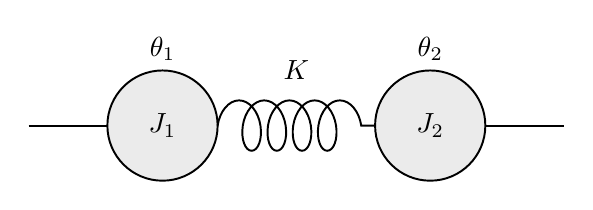
\begin{tikzpicture}[>={Stealth[length=2.6mm]}, line width=0.7pt]
  % inercia 1
  \draw (-3.4,0) -- (-2.4,0);
  \draw[fill=black!8] (-1.7,0) circle (0.7); \node at (-1.7,0) {$J_1$};
  \node[above] at (-1.7,0.7) {$\theta_1$};
  % resorte torsional K
  \draw[decorate, decoration={coil, aspect=0.6, segment length=3.2mm, amplitude=3.2mm}]
        (-1.0,0) -- (1.0,0);
  \node[above] at (0,0.45) {$K$};
  % inercia 2
  \draw[fill=black!8] (1.7,0) circle (0.7); \node at (1.7,0) {$J_2$};
  \node[above] at (1.7,0.7) {$\theta_2$};
  \draw (2.4,0) -- (3.4,0);
\end{tikzpicture}
\end{document}
